\documentclass[journal]{IEEEtran}
\usepackage{colortbl}
\usepackage{graphicx}
\usepackage{geometry}
\usepackage{float}
\usepackage[table,xcdraw]{xcolor}
\usepackage{amssymb}
\usepackage{amsmath}
 \usepackage{comment}
% Cite URL and break line
\usepackage{url}
\usepackage{breakurl}
\def\UrlBreaks{\do\/\do-}
%%
\usepackage{setspace}
\usepackage{slashbox}
\usepackage{flushend,cuted}
\usepackage{makecell,rotating,multirow,diagbox}
\usepackage{listings}
\usepackage[framed,numbered,autolinebreaks,useliterate]{mcode}
\hyphenation{op-tical net-works semi-conduc-tor}
%\setlength{\intextsep}{10mm}
%\setlength{\belowcaptionskip}{5mm}
% define the title
\author{Zhikun Zhu% <-this % stops a space
% <-this % stops a space
}
\title{Machine Learning Asisted Cognitive Radios}
\begin{document}
% generates the title
\maketitle
% insert the table of contents
% \tableofcontents
\begin{abstract}
%\boldmath
The abstract goes here.
\end{abstract}
\begin{IEEEkeywords}
IEEEtran, journal, \LaTeX, paper, template.
\end{IEEEkeywords}
\section{Week 1}
Below is what I have done this week:
\begin{itemize}
  \item Read through \cite{bkassiny2013survey}, which gives a detailed survey about how Machine learning techniques can be implemented in Cognitive Radios (CRs).
  \item Reviewed some machine learning techniques mentioned in the paper.
\end{itemize}
\subsection{The definiton of Cognitive Radios}
According to Haykin's paper \cite{haykin2005cognitive}, a CR is defined to be `\textsl{an intelligent wireless communication system that is aware of its environment and uses the methodology of understanding-by-building to learn from the environment and adapt to statistical variations in the input stimuli}'. And it is aimed to achieve two \textbf{objectives}:
\begin{itemize}
  \item Permanent reliable communications;
  \item Efficient utilization of frequency spectrum resources.
\end{itemize}
\subsection{How and what Machine learning techniques can be employed}
To perform its Cognitive tasks, a CR should be aware of its RF environment, where learning techniques can be applied to estimate the wireless channel characteristics and to determine the specific coding rate that is required to achieve a certain probability or error. And the problem of channel estimation is relatively simple and can be solved via estimation algorithms. However, problems become more complicated in the case of CRs and cognitive radio networks (CRNs) since the increase of degree of freedom.


\textbf{Unsupervised learning} may the best choice for CR which operating in alien RF environment, under which case, autonomous unsupervised learning algorithms permit exploring the environment parametres and self-adapting without any prior knowledge.


\textbf{Supervised learning} may be the best choice if CRs have perior knowledge about the environment.


Both supervised and unsupervised learning thchniques have been proposed for various learning tasks. supervised learning like Support Vector Machine (SVM) and neural networks can be used for CR applications. On the other hand, unsupervised learning such as Reinforcement Leanring (RL) can be used for Dynamic Spectrum Sharing (DSS).\\
\begin{figure}[H]
  \centering
   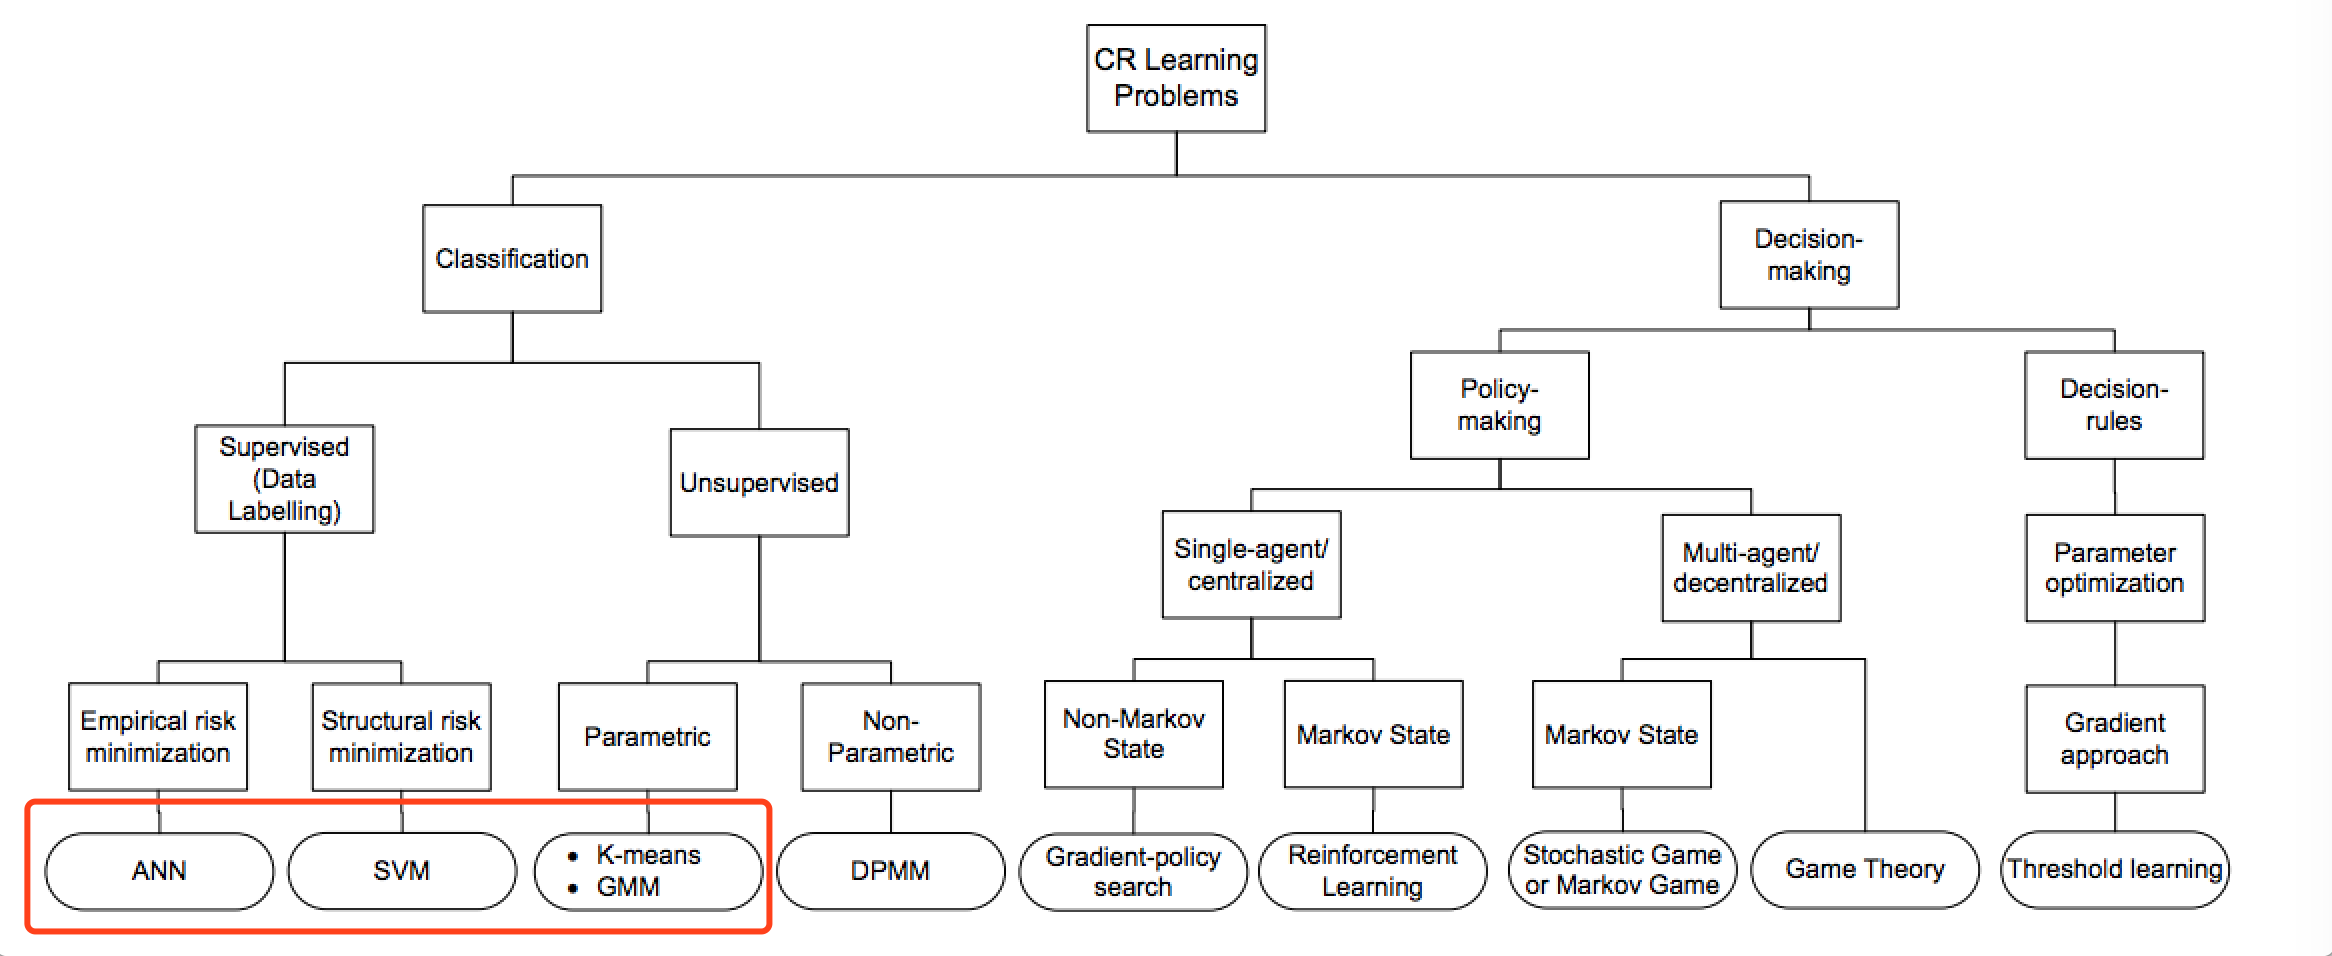
\includegraphics[width=1\textwidth]{CV_ML.png}

    \textsl{\caption{Typical problems in cognitive radio and their corresponding learning algorithms\cite{bkassiny2013survey}.}}

\end{figure}
\subsection{ANN \& SVM}
Figure.3 shows a basic Artifical Neural Network (ANN) with an input layer, a hidden layer and an output layer. There are also a bias for each layer which is not shown in the figure. Nodes in the ANN are called neuron. Each neurons in the output layer uses a nonlinear activation function. There are several activation functions and the choice usually related to the problem to be solved. The one mentioned in the paper called sigmod function is defined by:
\begin{equation}
  f(x) = \frac{1}{1+e^{-x}}
\end{equation}
The net output for each neuron at the output layer for the ANN defined in Figure.2 is:
\begin{equation}
  g_k(X) = f(\sum_{j=1}^{n_H}w_{jk}f(\sum_{i=1}^dw_{ji}x_i+w_{j0})+w_{k0})
\end{equation}
ANN is a supervised learning algorthms then it is trained by the target set. Here the error function is defined by:
\begin{equation}
  J(w) = \frac{1}{2}\sum_{k=1}^c(t_k-z_k)^2
\end{equation}
Then we can train the ANN by gradient descent, where $\Delta w = -\frac{\partial J}{\partial w}$. Since generally the ANN have more than one hidden layer, then, it is time consuming to calculate the gradient for each neuron by Equation.2. Hence, back-propagation (BP) is a popular method to train ANN, which employ chain rule to reduce the complexity of gradient calcluation.\\
\begin{figure}[H]
  \begin{minipage}[t]{0.5\linewidth}
    \centering
    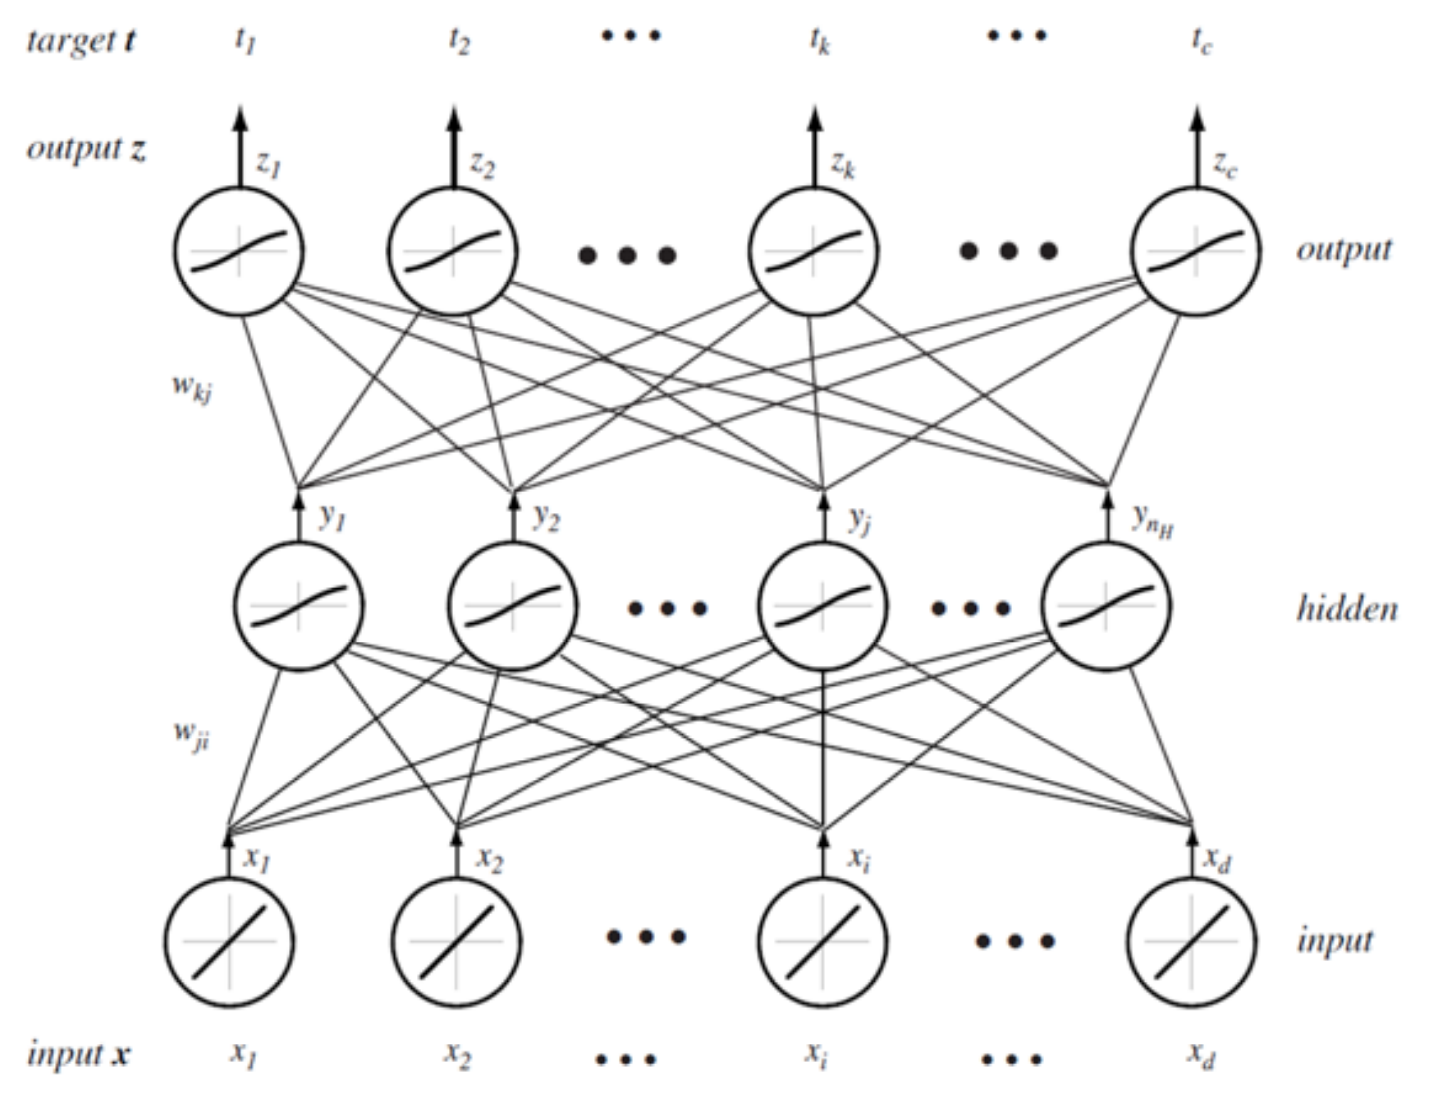
\includegraphics[width=2.2in]{ANN.png}
    \caption{Artifical Neural Network \cite{kate2017ANN}.}
  \end{minipage}
  \begin{minipage}[t]{0.5\linewidth}
    \centering
    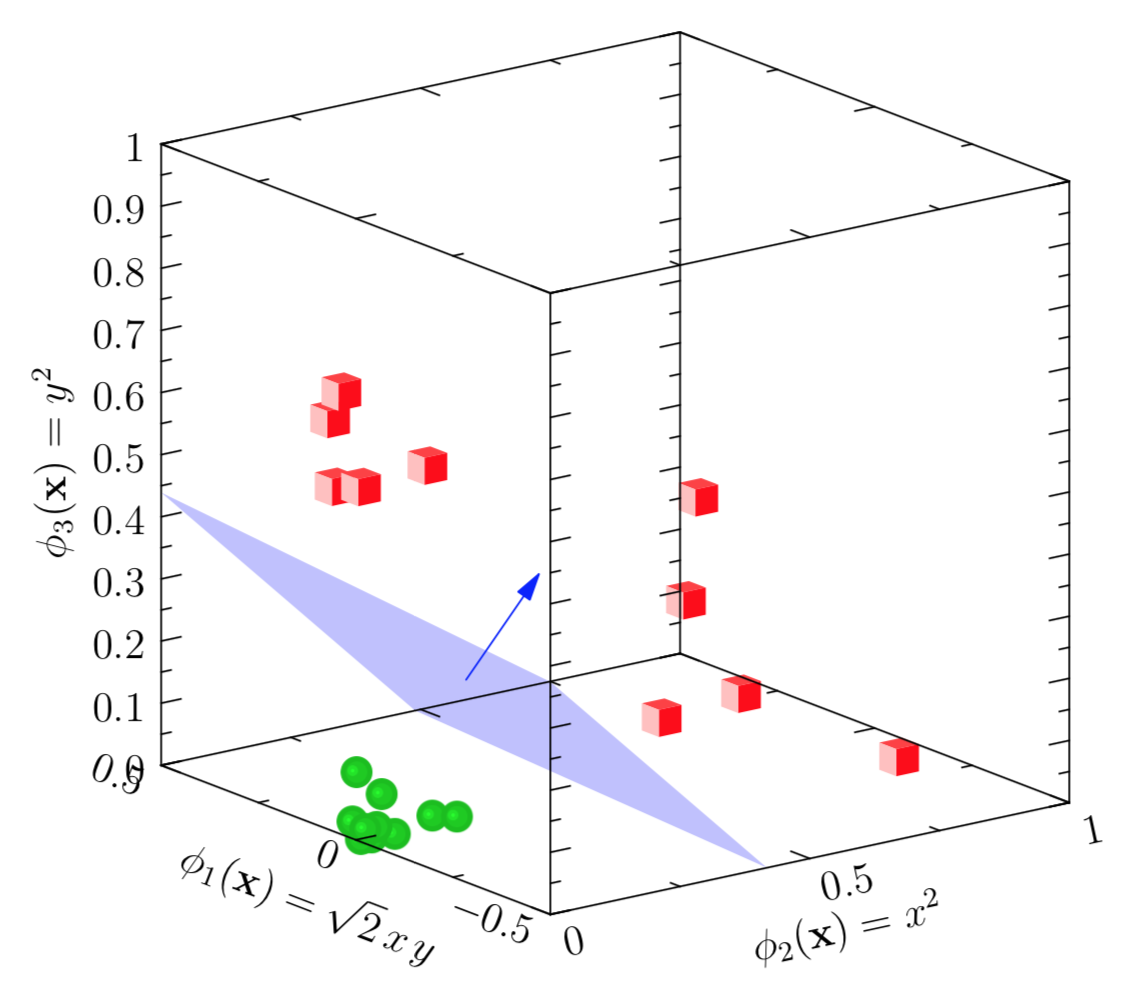
\includegraphics[width=2.2in]{SVM.png}
    \caption{Support Vector machine with hyperplane \cite{adam2017SVM}.}
  \end{minipage}
\end{figure}
Support Vector Machine, sometimes called maximum margin classifier, is a famous algorithm which used to solve classification problems. Basically it can only solve binary classifcations, but with some tricks (i.e. One-versus-One or One-versus-All), it can also handle multi-classification problems.


Suppose we have a weight vector $\textbf{w}$ and a bias $b $, the SVM is got by maximize the margin $m$:
\begin{equation}
  y_k\left(\frac{w^Tx_k}{\|w\| - b} \right) \geqslant m \qquad \forall \quad k = 0,2,...,N-1
\end{equation}
Define $\hat{w} = w/m\|w\|$ and $\hat{b} = b/m$, note that $\|\hat{w}\| = 1/m $. Then equation.4 becomes:
\begin{equation}
  y_k\left(\hat{w}^Tx_k-\hat{b} \right) \geqslant 1 \qquad \forall \quad k = 0,2,...,N-1
\end{equation}
Then, maximize margin m is equivalent to minimize $\|\hat{w}\|$, thus equivalent to minimize $\frac{1}{2}\|\hat{w}\|^2$, which is a quadratic programming (QP) problem. Applying Lagrange multipliers, and take the derivatives for both $\hat{w}$ and $b$ and substract them back to equation.5, the problems can turn into the dual form:
\begin{equation}
  \max \limits_{\alpha} \sum_{k=1}^P \alpha_k - \frac{1}{2}\sum_{k=1}^P\sum_{l=1}^P\alpha_k\alpha_l y_k y_lx_k^T x_l \qquad s.t. \sum_{k=1}^P\alpha_ky_k = 0 \quad \alpha_k \geq 0 \quad \forall  k = 0,1,...,N-1
\end{equation}
The dual form doesn't involve $w$ and involves only the dot product $x_k^T x_l$, which can be solved by kernel function and needn't to map the vector to higher dimension, which highly reduced the computation complexity.
\section{Week 2}
What I have done this week:
\begin{itemize}
  \item Read the paper matierial about cooperative communications of CR networks \cite{liang2013cooperative} (Haven't finsised yet).
  \item Reviewed the paper for week 1 and write the weekly report for both week 1 \& 2.
  \item Found a related paper \cite{o2017introduction} and read it for the following week.
\end{itemize}
\subsection{CR assisted cooperative communicaations}
According to \cite{liang2013cooperative}, there are three familiar structures of cognitive radios: \textbf{uderlay, overlay, and interweave networks}, which defined the different interaction between Primary users (PUs) and Cognitive Users (CUs).
\begin{itemize}
  \item \textbf{Underlay}: PUs support CUs to communicate under the circumstance that CUs' interference cannot affect PUs' communication quality.
  \item \textbf{Overlay}: Both CUs and PUs communicate using the same frequency spectrum and space and cooperative communication techniques employed. CUs act as a cognitive relay node (RN) in exchange for PUs' spectrum, time resource.
  \item \textbf{Interwave}: CUs and PUs can transmit simultaneously when there is a false hole detection of frequency spectrum by the sensor. Thus the transmit power is limited by the sensor's sensing range, instead of if there is interference.
\end{itemize}
In cognitive assisted cooperative communication network, \cite{liang2013cooperative} defined three types of categories: 1) cooperative communications between PUs, the classical cooperative networks; 2) Overlay, where PUs and CUs cooperate together, which have higher priority; 3) cooperation between CUs, which is a bit like category 1.


\subsection{Two relay strategies: AF \& DF}


Among different relay forwarding strategies, Amplify and Forward (AF) and Decode and Forward (DF) are two popular methods. In the amplify and forward mode, the relay only magnify the received signals (including signal and noise) and r-transmit it, whereas DF mode demodulates then re-modulates and send the signal.


Compared with the DF mode, the AF doesn't require calculation and has a small delay, but since the desired signal is amplified together with Gaussian white noise (AWGN), the SNR of the transmitted signal is higher than that of the DF mode. Besides, AF mode is more safe since the relay only need to amplify the received signal.


The SNR channel capacity equation for both AF and DF will be given in section week 3.

\subsection{The goal of paper \cite{liang2013cooperative}}
\begin{itemize}
  \item This paper is focused on overlay network.
  \item Aim to increase the data rate of CUs by utilizing the bandwidth supported by PUs and simultaneously maintian and even boost the throughput of PUs by using one of many CUs as a RN.
  \item Consider multiple PUs and CUs. Looking to find the best strategy that utilized the spectrum and time resources. Where the game theory introduced.
  \item One-way relay aided cooperative CR system: multiple CUs and a single PU.
  \item Novel two-way relay aided cooperative CR scheme: multiple CUs and two PUs.
  \item Two protocols in this scenario: Time Division Broadcast Channel (TDBC), with 3 time slots; Multiple Division Broadcast Channel (MABC), with only 2 time slots.
\end{itemize}


\begin{comment}
\begin{table}[htbp]\footnotesize
  \begin{center}
    \begin{tabular}{|c|c|c|c|}
      \hline
      Method & \begin{tabular}[c]{@{}l@{}}Bayesian\\ Boundary\end{tabular} & \begin{tabular}[c]{@{}l@{}}NN with\\ Training Set\end{tabular} & \begin{tabular}[c]{@{}l@{}}NN with\\ Test Set\end{tabular} \\ \hline
      Error  & 0.0701                                                      & \cellcolor[HTML]{C0C0C0}{0.0694}          & 0.0870                                                     \\ \hline
    \end{tabular}
  \end{center}
\caption{\textsl{Error rate comparison}}
\end{table}


\begin{table}[H]\footnotesize
  \begin{center}
    \begin{tabular}{|c|c|c|c|c|}
      \hline
      \backslashbox{\textbf{Row}}{\textbf{Col}}    & 1       & 2       & ... & 20      \\ \hline
      1    & x(1)    & x(2)    & ... & x(20)   \\ \hline
      2    & x(2)    & x(3)    & ... & x(21)   \\ \hline
      ...  & ...     & ...     & ... & ...     \\ \hline
      1480 & x(1480) & x(1481) & ... & x(1499) \\ \hline
    \end{tabular}
  \end{center}
  \textsl{\caption{FNN Training set.}}
\end{table}
\end{comment}


\section{Week 3: 21-03-2018}
What I have done this week:
\begin{itemize}
  \item Read an introduction book to Game theory \cite{barron2013game} to have an intuitive understanding of what is game theory. Despite the numberless models, game theory is composite of two primary divisions: cooperative and noncooperative games \cite{barron2013game}, which both can be utilized to solve the problem of resource allocation(i.e. frequency and time slots) in cognitive communications among multiple PUs and SUs.
  \item Nash equilibrium seems to be a freqneutly mentioned concept in game theory, so I read through materials to understand it.
  \item Modify the previous sections like misplace of citations and rewrite the sequence that directly abstract from the cited papers.
\end{itemize}
\subsection{What is a game?}
A game consider N players, each have a strategy that have been choosen at the begining of game, and each with a payof\/f to represent itself wins or loses.


\textbf{Zero sum game}. In Two-person zero sum game, whatever player 1 get, i.e. $a_{ij}$ as itself payof\/f, player 2 will have $-a_{ij}$ as itself payof\/f. Then, total payof\/f is a constant zero. Beside, suppose player 1 have M strategies and N for player 2. Then we can build a M-by-N matrix called payof\/f matrix for each player.


\textbf{Constant sum game}. Constant sum game is a broader group of zero sum game, where payof\/f for player 1 and 2 are $a_{ij}$ and $C - a_{ij}$, respectively. So, the sum payoff is a constant C, which will reduced to zero sum game when $C=0$. Then, such scenario can be considered as zero sum game to get the optimal result.


\textbf{Lower value of the game.} From row player's perspective, it assume that column's player try to minimize it cost over column \textsl{j}. That is, for each strategy row player have, it assume that column player will choose the corresponding strategy which minmize row player's payoff, then row player choose the strategy  \textsl{i} that maximize the payoff among all options suit such assumptions:
\begin{equation}
  v^- \equiv \max \limits_{i=1,2,...,m} \quad \min \limits_{j=1,2,...,n} a_{ij}
\end{equation}


\textbf{Upper value of the game.} The definition is conjugate to the lower value of the game since it is from the perspective of column player. Firstly, column player assume row player will choose the strategy that maximize itself payoff, then column player choose the strategy which have minimum value among all these strategies row player may choose.
\begin{equation}
  v^+ \equiv \min \limits_{j=1,2,...,n} \quad \max \limits_{i=1,2,...,m}  a_{ij}
\end{equation}


In summary, $v^-$ is the largest minimum and $v^+$ is the smallest maximum. Thus, $v^+ \geqslant v^-$.


\textbf{Saddle points}. Saddle point for a two-person game are the points in the payoff matrix which are the minimum for one column as well as the maximun for another column. According to \cite{barron2013game}, the precise definition of saddle points in \textbf{pure strategies} is:
\begin{equation}
  a_{ij^*} \leqslant a_{i^*j^*} \leqslant a_{i^*j} \qquad \forall i = 1,2,...,m \quad j = 1,2,...,n
\end{equation}
Saddle points means the maximum in one direction and the minimum in the other direction. Under the situation of pure strategies, \textbf{a game will have saddle point i.f.f}:
\begin{equation}
  v^- = \max \limits_{i} \min \limits_{j} \quad a_{ij} = \min \limits_{j} \max \limits_{i} \quad a_{ij} = v^+
\end{equation}

\subsection{Overlay cognitive cooperative network}
Under the scenario of overlay, CU act as a relay node in exchange for PU's spectrum resource. Hence, the message signal transmitted by source node will be relayed by the relay node, then it can be considered as a MISO system and diversity gain can be achieved. Suppose that the noise for channel $h_{sd}$, $h_{sr}$ and $h_{rd}$ have the same power spectrum, $N_0$. And the transmit power for Tx and RN are $P_s$ and $P_r$, respectively. Then the SNR for the channel between source node, relay node, and destination node are:
\begin{equation}
 \gamma_{sr} = \frac{P_s|h_{sd}|^2}{N_0} \qquad \gamma_{rd} = \frac{P_rd|h_{rd}|^2}{N_0} \qquad \gamma_{sd} = \frac{P_s|h_{sd}|^2}{N_0}
\end{equation}
According to \cite{hasna2003end}, the overall Signal-to-Noise Ratio (SNR) for AF mode is:
\begin{equation}
\gamma = \frac{\gamma_{sr}\gamma_{rd}}{\gamma_{sr}+\gamma_{rd}+1}
\end{equation}
Here is only the S-R-D route, and if we consider the S-D route together, we can get the final channel capacity:
\begin{equation}
C_{PU}^{AF}  = \frac{W_1}{2} \log_2(1 + \gamma + \gamma_{sd}) = \frac{W_1}{2} \log_2(1 + \frac{\gamma_{sr}\gamma_{rd}}{\gamma_{sr}+\gamma_{rd}+1} + \gamma_{sd})
\end{equation}


For DF mode, we achieve diversity gain by consider channel $h_{rd}$ and $h_{sd}$ together, combining with the end-to-end SNR for DF relay, we can get the channel capacity:
\begin{equation}
C_{PU}^{DF} = \frac{W_1}{2} \min\{\log_2(1 + \gamma_{sd}+\gamma_{rd}),\quad \log_2(1 + \gamma_{sr})\}
\end{equation}
\begin{figure}[H]
    \centering
    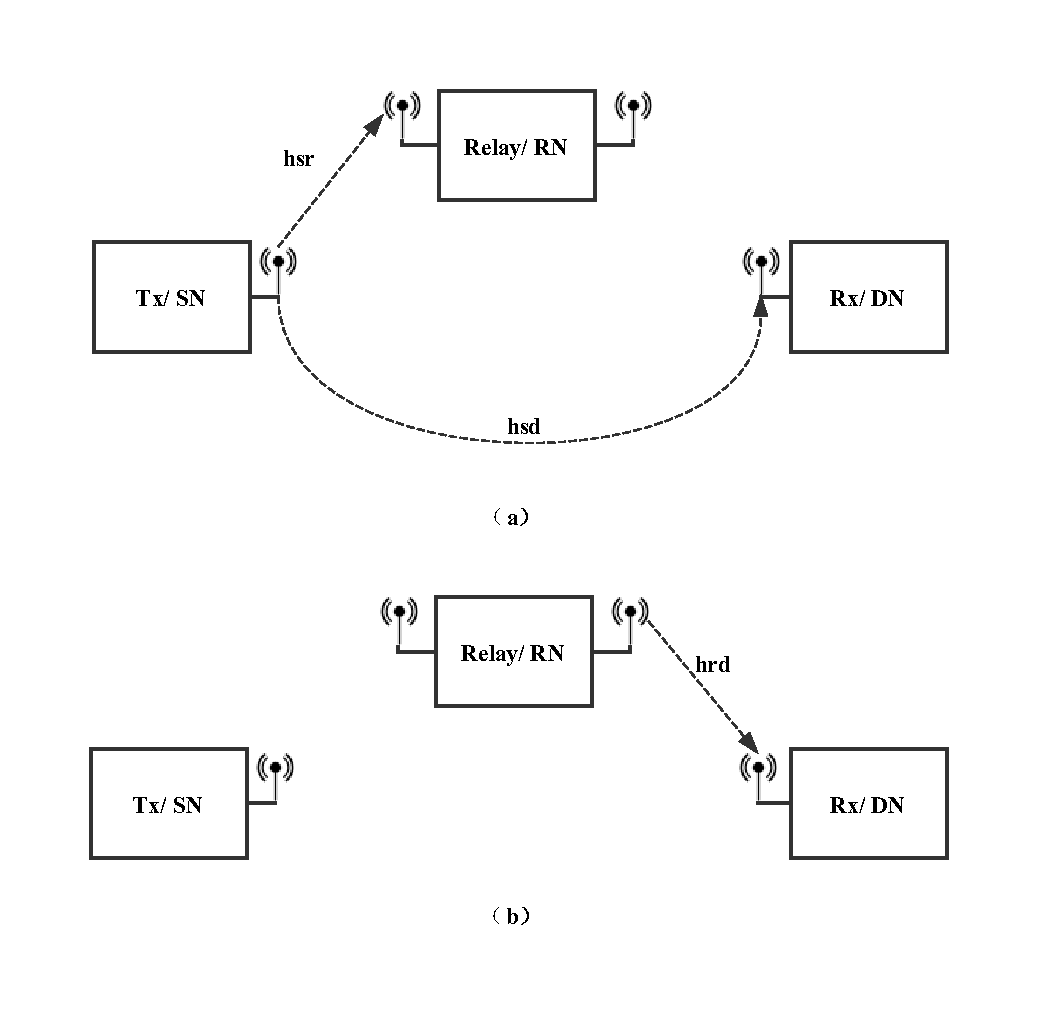
\includegraphics[width=3in]{relay.pdf}
    \caption{Cognitive radio assisted relay network.}

\end{figure}

\section{Week 4 \& 5: 9-04-2018}

\subsection{Nash equilibrium}
A game contains N players (rational entities) and each player have a set of actions $A_i$ and utility functions $U_i$:
\begin{equation}
  G = (\mathcal N, (\mathcal A_i)_{i \in \mathcal N},(U_i)_{i \in \mathcal N}) \qquad \mathcal N = \{1,...,N\}
\end{equation}
Generally, the utility function $U_i$ for player i is a function of strategies selected by all player. Here we use $U_i(a_i,a_{-i})$ to denote it, where $a_i$ is the strategy selected by $i$ and $a_{-i}$ is strategies selected by other players excepted i. Under the circumstance of pure strategies and all players aim to maximun itself utility functions. A Nash equilibrium is defined as a point where the utility function for each player does not increase givn that only itself change strategy. Mathmatically, a strategy set $(a_1^*,a_2^*,...,a_N^*) \in \mathcal A$ is said to be a Nash equilibrium if:
\begin{equation}
  U_i(a_i^*,a_{-i}) \geq U_i(a_i^\prime,a_{-i}) \quad \forall i \in \mathcal N, \quad \forall a_i^\prime \in \mathcal A_i,
\end{equation}
\subsection{Information entropy}
We begin by consider how much information we got if we received a random variable x, which have a distribution p(x). If we know something gonna to be happen, then we receive no information, but if we know something with a very low probability to be happen, then we receive much information. Then, the information we received have something to do with it's distribution \cite{nasrabadi2007pattern}. We use h($\cdot$) to denote the information we received. Now consider two independent incidence x and y. We expect to have $p(x,y) = p(x) \cdot p(y)$ and $h(x,y) = h(x) \cdot h(y)$. Then logarithm comes to our mind:
\begin{equation}
  h(x) = -\log_2(p(x))
\end{equation}
Then, the average information we got by transmitting x is got by take expectation with respect to p(x):
\begin{equation}
  H(x) = -\sum \limits_x p(x)\log_2(p(x))
\end{equation}
The quantity is called the entropy of random variabe x and with unit \textsl{bits}. Shannon stated that the entropy is the lower bound on the number of bits need to be transmit the state of random variable.


The term \textbf{Cross Entropy} is the amount of information that calculated by distribution q(x) instead of real distribution p(x):
\begin{equation}
  H(x) = -\sum \limits_x p(x)\log_2(q(x))
\end{equation}
There are also term \textbf{Relative Entropy (KL diver- gence)} used to denote the additional amount of information needed to transmit x using distribution q(x) insted of real distribution p(x):
\begin{equation}
  H(x) = -\sum \limits_x p(x) \log_2(\frac{q(x)}{p(x)})
\end{equation}
The cross entropy can be used as cost function in machine learning algorithm since the lower it is the better the strategy compared with optimal. And the relative entropy can be used to compare the difference of different strategy.

\section{Week 6: 19-04-2018}
\subsection{Reinforcement learning}
As noticed, reinforcement learning (RL) permits a agent/ learning machine to learn by interacting with the environment \cite{sutton1998reinforcement} without any prior knowledge, which is the key advantageous of such technique because the nature of the radio frequency environment is unknow. Thus, this technique empower the agent to learn without supervision. According to Fig.1, decision making process in CR is a process that enable CR to interact with the environment and such process can be improved by learning, thus making RL a promising choice for this task. RL has been used for dynamic spectrum access in cognitive radio network (CRN) \cite{yau2010applications},

For each state $s_i$, a reinforcement learning machine have an action $a_i$ based on the actor/ policy $\pi_\theta (s)$, and got a reward from the environment $r_i$. The interaction process between learning machine and environment can be considered as a Markov decision process (MDP), where the state $s_{t+1}$ only determined by previous state $s_t$ and action $a_t$:
\begin{equation}
  p(s_{t+1}|s_t,a_t,s_{t-1},a_{t-1},...,s_{0},a_0) = p(s_{t+1}|s_t,a_t)
\end{equation}

For a given policy $\pi_\theta (s)$ and a given terminal state $s_T$, the trajectory of MDP is defined as $\tau = \{s_0,a_0,s_1,a_1,...,s_T,a_T\}$. The  cumulative reward $R(\tau)=\sum \limits_{n=1}^T r_n$ is what the training method need to maximize. And for those without terminal state, especially the case for cognitive radio, discounted future reward is defined as $R(\tau)=\sum \limits_{n=t}^T \gamma^{n-t}r_n$. Generally, the  cumulative reward $R(\tau)$ is a conditional random variable of policy $\pi_\theta$. The aim for training is to maximize the reward expection $\overline{R}_\theta$. However, conditional probability density function $p(\tau|\theta)$ is unreachable, where we use Monte Carlo method to approximate $\overline{R}_\theta$:
\begin{equation}
  \overline{R}_\theta = \sum \limits_\tau R(\tau)p(\tau|\theta) = \frac{1}{N}\sum \limits_{n=1}^N  R(\tau^n)
\end{equation}

The learning problem is then become
\begin{equation}
  \theta^* = \arg \max \limits_\theta \overline{R}_\theta
\end{equation}
There are two ways in solving the problem under the assumption of Markov state, policy gradient and Q-learning. And gradient policy search is proposed for non-Markov state environment.

\bibliographystyle{ieeetr}
\bibliography{cite}
\end{document}
